%% \documentclass[twoside]{report}
\documentclass[a4paper]{report}


\usepackage[sc]{mathpazo}
\usepackage[T1]{fontenc}
\usepackage[utf8]{inputenc}
\usepackage[frenchb]{babel}
\linespread{1.05}
\usepackage{microtype}

%% \usepackage[hmarginratio=1:1,top=32mm,columnsep=20pt]{geometry}
%% \usepackage{multicol}
\usepackage[hang, small,labelfont=bf,up,textfont=it,up]{caption}
\usepackage[top=4cm, bottom=4cm, left=4cm, right=4cm]{geometry} 
\usepackage{booktabs}
\usepackage{float} 
\usepackage{hyperref}

\usepackage{graphicx}
\usepackage{listings}

%% Usefull for \FloatBarrier
\usepackage{placeins}

\usepackage{lettrine}
\usepackage{paralist}
\usepackage{setspace}

\usepackage{abstract}
\renewcommand{\abstractnamefont}{\normalfont\bfseries}
\renewcommand{\abstracttextfont}{\normalfont\small\itshape}

\usepackage{titlesec}
%% \renewcommand\thesection{\Roman{section}}
%% \renewcommand\thesubsection{\Roman{subsection}}
\titleformat{\chapter}[hang]{\bf\huge}{\thechapter}{2pc}{} 
%% \titleformat{\section}[block]{\large}{\textbf\thesection.}{1em}{\textbf}
%% \titleformat{\subsection}[block]{\large}{\thesubsection.}{1em}{}

\newcommand{\myfig}[4] {
  \FloatBarrier
  \begin{figure}[!h]
    \centering
    \includegraphics[scale=#1]{#2}
    \caption{#3}
    \label{#4}
  \end{figure}
  \FloatBarrier
}

\setcounter{tocdepth}{3}

%----------------------------------------------------------------------------------------
%% TITLE SECTION
%----------------------------------------------------------------------------------------

\title{\vspace{+0cm}\fontsize{24pt}{10pt}\selectfont\textbf{Monitoring du noyau Linux sur une architecture NUMA}}

\author{
\large
\textsc{Kévin Gallardo, Eric Lombardet, Pierre-Yves Péneau}\\[2mm] 
\normalsize Université Pierre et Marie Curie - Jussieu - Paris VI
\vspace{-5mm}
}
\date{}

%----------------------------------------------------------------------------------------
%MACROS
%----------------------------------------------------------------------------------------

\newcommand{\ig}[1]{\begin{figure}[H]\begin{center}\includegraphics[scale=0.5]{#1.png}\end{center}\end{figure}}
\newcommand{\benum}{\begin{enumerate}}
\newcommand{\eenum}{\end{enumerate}}
\newcommand{\bitem}{\begin{itemize}}
\newcommand{\eitem}{\end{itemize}}
\newcommand{\PMC}{Performance Monitoring Counter }
\newcommand{\IBS}{Instruction Based Sampling }
\newcommand{\lap}{Local APIC }
\newcommand{\ioap}{IO_APIC }
\newcommand{\lwp}{LightWeight Profiling }



%----------------------------------------------------------------------------------------
%% HEADER STYLE
%----------------------------------------------------------------------------------------
\usepackage{fancyhdr}
\pagestyle{fancy}
% \fancyfoot{}
\fancyhead[L]{Monitoring du noyau Linux sur une architecture NUMA}

%----------------------------------------------------------------------------------------
\begin{document}
  \maketitle
  \newpage

  \tableofcontents
  \newpage

  \setcounter{page}{0}
  \thispagestyle{empty}
  \begin{abstract}
    \centering
    \noindent L’essor de l’informatique en nuage a permis aux administrations et entreprises
de stocker d’énormes jeux de données. Aujourd’hui, l’un des goulots
d’étranglement majeurs pour les performances de traitement de ces données est le
système d’exploitation de chaque machine. Les systèmes actuels ne peuvent pas
gérer efficacement les applications intensives en données car ils ne disposent
pas d’une vue unifiée des ressources utilisées, ce qui les empêche de déterminer
des stratégies efficaces pour le placement des tâches/données sur les ressources
matérielles. Une meilleure gestion des ressources permettrait une forte
réduction du nombre de machines nécessaires aux traitements des données.

L’implémentation de sondes dans le noyau Linux permettrait d'identifier les
ressources physiques et logicielles les plus sollicitées par les processus. Les
informations remontées par ces sondes peuvent ensuite permettre de commencer à
définir des stratégies de placement des tâches et des données prenant en compte
à la fois la topologie de la machine et l’utilisation effectives des ressources
par les tâches.

  \end{abstract}
  
  \begin{onehalfspace}
  \chapter{Introduction}

  \lettrine[nindent=0em,lines=3]{L} es systèmes multicoeurs modernes sont
  maintenant basés sur l'architecture NUMA (Non Uniforme Memory Access). Avec un
  système NUMA, les coeurs des processeurs sont regroupés en noeuds. Chaque
  noeud possède un contrôleur mémoire et est interconnecté avec les autres
  noeuds de la machine.

  \begin{figure}[H]
    \centering
    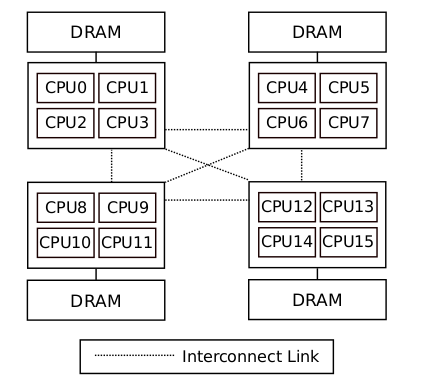
\includegraphics[scale=0.35]{img/numa_arch.png}
    \caption{Un système NUMA avec 4 noeuds et 4 coeurs par noeud}
    \label{f:numa_arch}
  \end{figure}

  Du fait des temps d'accès mémoire non uniforme, tout le défi des systèmes
  tournant sur cette architecture est la répartition des données et des
  traitements. En effet, la principale cause de latence n'est pas due au
  \textbf{temps de traitement des données}, mais au \textbf{temps d'accès aux
    données}. Ces accès coûtent entre 10\% et 40\% de temps supplémentaire par
  rapport aux accès locaux.\cite{Lepers2014} Dans une configuration idéale,
  chaque coeur irait chercher ce dont il a besoin dans la mémoire contrôlée par
  le noeud dans lequel il se situe. Ainsi, les demandes d'accès distant seraient
  réduites à néant, et il n'y aurait aucune latence due aux échanges entre les
  noeuds. Nous allons voir que cet idéal est très difficile, voire impossible à
  obtenir. Néanmoins, il est possible de s'en approcher, en mettant au point des
  algorithmes de répartitions de plus en plus efficaces. La création de ces
  algorithmes nécessite une connaissance approfondie du noyau: comment gère-t-il
  la création des threads, où sont-ils placés, quelles sont les pages mémoires
  accédées le plus souvent, par quels noeuds sont-elles contrôlées\ldots C'est
  en collectant un maximum de renseignements sur ces différents points (et de
  nombreux autres) que l'on pourra être en mesure d'affiner les solutions de
  répartition de charge. Cette étape de monitoring sera le sujet principal de ce
  projet de master. Nous allons devoir lire et comprendre le fonctionnement à
  très bas niveau du noyau, puis le modifier en utilisant divers outils de
  gestions d'évènements avec des bibliothèques comme IBS\footnote{Instruction
    Base Sampling, une technologie développée par AMD uniquement sur les
    processeurs Opteron} afin de préparer l'étape de réflexion pour la création
  d'algorithmes.

  \chapter{Architecture des ordinateurs}

  \lettrine[nindent=0em,lines=3]{N} ous allons dans un premier temps revenir sur le fonctionnement des
  ordinateurs indépendement de l'architecture considérée. Ainsi, les différents
  concepts seront expliqués dans leur généralités avant d'exposer les
  spécificités de l'architecture NUMA. Cette partie nous permettra de faire un
  bilan général des connaissances acquises lors des modules d'architecture et de
  noyau lors de cette année.


  \section{Principes généraux}

    \subsection{Le processeur}

    Le processeur est le coeur de l'ordinateur.  Son rôle est d'effectuer tous
    les calculs, lectures et écritures sur les données. Un processeur est
    cadencé à une certaine vitesse qui se mesure en cycle et qui varie selon les
    modèles.. À chaque cycle, le processeur est chargé d'aller chercher une
    instruction dans la mémoire, la décoder et l'exécuter.

    \subsubsection{Les caches}

      L'accès à la mémoire est une opération très couteuse, entre 100 et 2000
      cycles\cite{Lepers2014}. Afin d'accélérer ce processus, les ingénieurs ont
      créé les mémoires cache, ou plus communément caches. Les caches sont une
      zone mémoire de taille infiniment inférieure que la mémoire principale
      (entre 4Ko et 12Mo) mais en contrepartie beaucoup plus rapide d'accès (de
      3 à 5 cycles pour les caches de premier niveau) du fait de leur
      composition matérielle. Il peut y avoir plusieurs niveaux de cache, comme
      on le voit sur la figure ~\ref{f:cacheorga}.

      \myfig{0.5}{img/cacheorga.png}{Schéma de l'organisation des caches}{f:cacheorga}

      Chaque niveau de cache contient une partie des données de la mémoire
      RAM. La construction des caches se base sur deux grandes notions en
      architecture: la \textbf{localité spatiale} et la \textbf{localité
        temporelle}. La localité spatiale est une loi disant que si une donnée
      est accédée à une adresse A, il existe une très grande probabilité que la
      prochaine donnée à vouloir être accédée par le proceseur soit à l'adresse
      A+1. Cette loi se base sur le principe de la \textbf{séquentialité du
        stockage des données}. La localité temporelle nous dit quant à elle que
      si une donnée est accédée à un instant T, elle sera très probablement
      accédée de nouveau dans un temps futur très proche. Afin d'accélérer
      encore plus le traitement des caches de premiers niveaux, le cache L1 est
      coupé en deux parties: une contenant les identifiants d'instructions (les
      branchement, chargements\ldots) à charger, et l'autre les données
      relatives à ces instructions.

      Prenons une configuration simple avec un seul niveau de cache. Lorsque le
      processeur demande d'accéder à une donnée, il va maintenant le demander au
      cache et non directemment à la mémoire princiaple. Si le cache possède
      cette information il va déclencher un signal de \textbf{Cache Hit} et
      répondre au processeur. Dans le cas inverse, il va déclencher un signal de
      \textbf{Cache Miss}. Il va ensuite devoir accéder à la mémoire pour
      obtenir l'information demandée par le processeur et, en utilisant les lois
      de localité spatiale et temporelle évoquées précédemment, il va rapatrier
      les $X$ données suivant celle initialement demandée. Ainsi, pour les $X$
      prochains accès, il est très probable que le processeur obtiendra
      directement du cache ce qu'il veut, et les performances auront été
      significativement améliorées.

      Ce fonctionnement est le même si l'on ajoute plusieurs niveaux de cache,
      comme sur la figure ~\ref{f:caches}

      \myfig{0.37}{img/caches.png}{Schéma des niveaux caches d'un processeur}{f:caches}

      Le cache L3 est le plus gros, et il est généralement partagé en les
      processeurs. Les cache L1 est toujours local à un coeur. Les caches L2
      sont généralement locaux ou alors peuvent être partagés entre coeurs. Les
      caches de niveaux L3 sont eux généralement partagés entre les processeurs.

    \subsection{La mémoire}

      Nous avons précédement évoqué les accès mémoire sans rentrer dans les
      détails. En effet, la gestion des adresses est un processus assez
      complexe. Lorsque l'on parle de mémoire, il est important de différencier
      la mémoire physique de la mémoire virtuelle. La mémoire physique est,
      comme son nom l'indique, physiquement présente dans la machine. C'est que
      qu'on appelle les \og barettes de RAM\fg. La mémoire virtuelle est une
      couche d'abstraction de la mémoire physique, et c'est cette abstraction
      que le système d'exploitation voit et manipule. Ainsi, à chaque
      instruction nécessitant un accès, le processeur est obligé d'effectuer une
      traduction d'adresse. Cette opération est effectuée par l'\textbf{Unité de
        Gestion Mémoire}, ou \textbf{MMU} (Memory Management Unit). La MMU fait
      partie intégrante du CPU, bien que sur certains modèles elle soit sur un
      circuit séparé.\newline

      \myfig{0.5}{img/mmu2.png}{Schéma des communications entre le processeur et
        la MMU}{f:mmu2}

      La mémoire physique est découpé en partie logique appelées pages ou
      segments, selon le type de découpage. De nos jours les mémoires sont à la
      fois paginée et segmentée pour des raisons de performances. Un segment est
      un espace mémoire de taille variable, alors qu'une page a une taille fixe
      (généralement 4Ko). Toutes ces données sont stockées et gérées par le
      système d'exploitation dans la \textbf{table des pages}. Sur les machines
      x86-64, la table des pages est composée de quatre niveaux d'indirections
      (figure ~\ref{f:tdp}). Chaque entrée dans les trois premiers niveaux
      redirige vers le niveau suivant. L'entrée dans le dernier niveau est
      l'adresse de l'espace dans la mémoire physique. Afin de réaliser cette
      traduction, les adresses physiques sont coupées en cinq parties
      distinctes. Les quatres premières indiquent les indexes dans les niveaux
      d'indirection. La dernière partie contient l'offset de la donnée dans
      l'espace physique.
    
      \myfig{0.3}{img/tdp.png}{Découpage d'une adresse virtuelle en niveaux
      d'indirection}{f:tdp}

      Un des composant essentiel à la MMU est le \textbf{Translation lookaside
        buffer} (TLB). Ce composant agit comme un cache pour les accès
      mémoire. Il mémorise les derniers accès correspondant aux dernières pages
      auxquelles le processeur a dû accéder, permettant d'améliorer grandement
      les temps d'accès à la mémoire. La MMU, via le TLB connait donc toutes les
      équivalences entre adresse virtuelles et physiques.


      Voici une illustration représentant les échanges entre les processeurs,
      les différents niveaux de caches et la MMU et la mémoire RAM. Ici il n'y a
      que deux niveaux de caches et le deuxième est partagé entre les
      processeurs.
    
      \myfig{0.65}{img/cache_mmu_global2.jpg}{Schéma des interactions concernant
        les adresses et les données entre les différents composant d'un
        ordinateur}{f:memory}


    \subsection{Limites}
  
      Le type d'architecture présenté ici est utilisé partout dans nos machines
      à l'heure actuelle. Le besoin de recourir à d'autres solutions se cantonne
      uniquement à des utilisation particulière des ordinateurs. Prenons un
      serveur réalisant une quantité de calcul énorme à la minute. Comment
      réagira le contrôleur mémoire à toutes ces demandes d'accès simultannées ?
      Si ce même serveur à maintenant besoin d'effectuer un grand nombre
      d'entrées/sorties sur le disque dur, comment pouvoir garantir efficacité ?
      C'est dans cette optique qu'on été pensée les architectures NUMA: pouvoir
      répondre à ces problématiques particulières qui ne correspondent pas à
      celle du grand public.

\newpage

  \section{L'architecture NUMA}
    
    \textit{Dans cette partie nous détaillerons uniquement l'architecture de la
      machine que nous avons eu à notre disposition durant ce projet. Les
      concepts sont les mêmes sur d'autres machines NUMA, seuls les
      caractéristiques technique ou les méthodes d'implémentation diffèrent. La
      machine en question est appelé \og Magny Cour\fg et est produit par le
      constructeur américain
      AMD.\footnote{http://products.amd.com/pages/optoeroncpudetail.aspx?id=644}\newline}


    L'architecture NUMA a été pensée dans le but d'accélérer la vitesse de
    traitement de l'information par les machines ayant de gros besoin en
    ressources. Cette amélioration est rendue possible grâce à différents
    concepts que nous allons détailler dans par la suite.

  \subsection{Les noeuds}

    L'intérêt et la puissance de cette architecture repose sur la notion de \og
    noeud\fg. Un noeud est un ensemble de coeurs de processeurs regroupés sur
    une même puce. Chaque noeud contient un certain nombre de coeurs d'un
    processeur sur une puce, et celles-ci sont assemblées par deux sur un
    composant appelé \textbf{Multichip Module}, ou MCM. Notre machine dipose de
    quatre processeurs AMD Opteron 6172 de douze coeurs chacun. On a donc quatre
    MCM, contenant douze coeurs chacun, répartis en deux noeuds de six
    coeurs.\newline

    Les différents noeuds sont interconnectés entre eux via des bus appelés
    \textbf{liens Hypertransport} (HT links) et possèdent, selon les machines,
    un certain nombre de contrôleurs mémoire et d'entrées/sorties. Nous
    détaillerons par la suite les différentes caractéristique de ces
    périphériques. Sur notre machine, chaque noeuds est composé de quatre liens
    Hypertransport, deux contrôleurs d'accès mémoire, et certain ont un
    contrôleur d'entrées/sorties,

    \myfig{0.4}{img/mcm.png}{Illustration d'un MultiChip module}{f:mcm}

  \subsection{La communication entre les noeuds}

    La techonologie des liens Hypertransport permet l'interconnexion entre
    processeurs. Développée depuis 2001, elle est principalement utilisée par
    AMD dans ses machines NUMA mais également dans les systèmes
    MIPS\footnote{Microprocessor without Interlocked Pipeline Stages} les plus
    récents. Dans notre machine, il existe deux type de liens HT, la différence
    étant leur capacité de transport:

    \begin{itemize}
      \item[HT3 x8:] bande passante maximale de 6.4GB/s. 2.8GB/s obervés sur notre
      machine\cite{Lepers2014}
      \item[HT3 x16:] bande passante maximale de 25.6GB/s.De 3GB/s à 6.6GB/s sur
      notre machine\cite{Lepers2014}
    \end{itemize}

    Au sein d'un MCM, les noeuds sont reliés entre eux via un lien HT3 x8 et un
    lien HT3 x16. Les noeuds entre MCM sont connectés entre eux de la même
    manière. Néanmoins, tous les noeuds ne sont pas reliés entre eux, créant
    ainsi une \textbf{toologie} particulière pour la machine considérée. Comme
    le montre l'illustration ~\ref{f:topo} issue de la documentation officielle
    du Magny Cour, on voit que les couples de noeuds \{P1,P6\} et \{P2-P5\} ne
    sont pas reliés sur notre machine.

    \myfig{0.6}{img/topo.png}{Schéma de la topologie du \textit{Magny Cour}}{f:topo}

    Les communciations sur les liens HT se font par
    paquets\cite{CacheHierarchy}. Ils sont uniformes et comprennent un header
    contenant l'émetteur et le récepteur de la requête. Pour chaque couple de
    MCM, un noeud est défini comme étant le routeur. Si un noeud a besoin
    d'accéder à une donnée dont il connait le propriétaire mais n'est pas
    directement connecté à lui, alors il passera par le noeud routeur afin de
    satisfaire sa demande.


  \subsection{Les contrôleurs d'entrées/sorties}

    L'illustration ~\ref{f:topo} nous montre également une des particularité du
    Magny Cour: la disposition des contrôleurs d'entrée/sortie. Ces derniers ont
    été placés uniquement sur les noeuds P1 et P5. Cette disposition permet une
    diminutation de la latence des échanges entre les noeuds mais peut être
    source de problème si les applications solicitant la machine doivent faire
    beaucoup d'entrées/sorties. C'est notamment pour cela qu'il est important de
    savoir quelles applications seront utilisées sur une machine avant de
    procéder à l'achat. Dans la documentation du Magny Cour, il est dit que
    cette machine a été étudiée pour du calcul haute performance et non pour des
    entrées/sorties.

  \subsection{Les accès mémoire}

    Dans notre configuration, chaque noeud possède deux contrôleurs mémoire, et
    donc une partie de la mémoire physique. Le découpage est fait équitablement
    de la façon suivante: le noeud numéro 1 possède la partie basse de la
    mémoire, le noeud numéro 2 la partie suivante, et ainsi de suite jusqu'a
    noeud numéro 8.

    L'accès par un noeud à une donnée présente dans sa partie de la mémoire est
    appelé \textbf{accès local}. Dans le cas contraire, c'est un \textbf{accès
      distant}. Les accès distants sont possibles grâce au HT Links. Ces
    derniers sont chargés d'assurer la communication entre les noeuds, que ce
    soit pour les demandes d'accès aux données que pour la cohérence des
    caches. Le coup d'un accès distant est environ 15\% plus cher qu'un accès
    local.\cite{Lepers2014}

    TOFINISH

  \subsection{Les caches}

    Comme tout processeur, notre machine possède différents niveaux de cache:
    L1, L2 et L3. Les caches L1 et L2 sont locaux aux CPU, tandis que les caches
    L3 sont partagés. Leur taille est respectivement de 64Kb, 512K et 6Mb. Afin de 

    \subsubsection{La cohérence des caches}

      
    

  %% \subsection{Étude du contexte}

  \lettrine[nindent=0em,lines=3]{L}e but de se projet sera dans un premier temps
  de mettre en place une infrastructure de compilation, de test et d'exécution
  d'un noyau Linux. La seconde partie du projet sera de comprendre comment
  fonctionne le noyau Linux au niveau de la mémoire, notamment pour la gestion
  des pages (emplacement, taille), et au niveau des processeurs pour le
  placement des threads et me parallélisme. Ensuite, il faudra se plonger dans
  la lecture du code et sa modification aux endroits adéquats en utilisant des
  technologies comme IBS où les hardware counters pour obtenir des informations
  précises sur la gestion des points évoqués ci-dessus. Enfin, pour tester ce
  noyau avec nos modifications, nous utiliserons la machine virtuelle et gdb
  pour le débugage.
  %% TODO: changer débugage par autre chose

  \subsubsection{Infrastructure}
    Dans cette partie, nous allons détailler l'infrastructure dont nous
    disposons et celle que nous avons mise en place pour ce projet. Notre avons
    à notre disposition une machine AMD Opteron 6172 composée de quatre
    processeurs à douze coeurs chacun cadencés à 2,1GHz et répartis en 8 noeuds
    avec 32G de mémoire vive. L'architecture des noeuds est la
    suivante\footnote{Source: \textit{Improving performance on NUMA systems},
      Baptiste Lepers}:

    %% TODO: vérifier l'archi à la main (méga chaud et méga long)

    %% node   0   1   2   3   4   5   6   7 
    %%   0:  10  16  16  22  16  22  16  22 
    %%   1:  16  10  16  22  22  16  22  16 
    %%   2:  16  16  10  16  16  16  16  22 
    %%   3:  22  22  16  10  16  16  22  16 
    %%   4:  16  22  16  16  10  16  16  16 
    %%   5:  22  16  16  16  16  10  22  22 
    %%   6:  16  22  16  22  16  22  10  16 
    %%   7:  22  16  22  16  16  22  16  10

    \begin{figure}[H]
      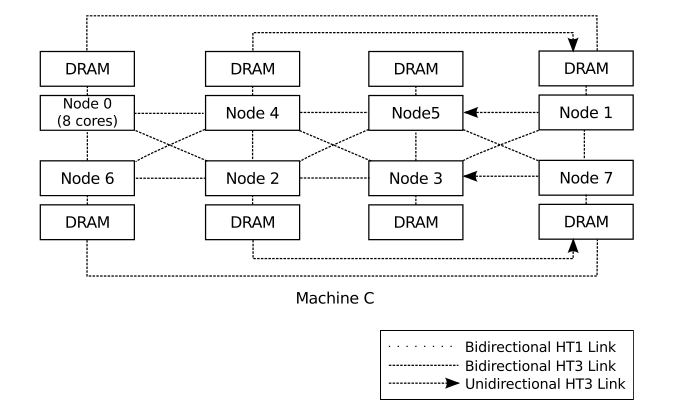
\includegraphics[scale=0.4]{img/numa_topology.png}
      \caption{Topologie de la machine 6172}
      \label{f:numa_topology}
    \end{figure}

    Sur cette machine, nous avons utilisé l'hyperviseur qemu, avec son extension
    kvm pour afin d'optimiser l'émulation. Afin d'améliorer encore plus cette
    dernière, nous avons utilisé le logiciel virt-manager qui détecte
    automatiquement la configuration matérielle de machine hôte et configure la
    machine virtuelle en conséquence. Cette configuration est à notre avis très
    réaliste puisqu'elle est capable d'activer/désactiver des options CPU comme
    la gestion d'IBS où l'hypervision. Un des autres avantage de virt-manager
    est que l'on peut sauvegarder la configuration dans un fichier, et pouvoir
    ainsi l'exporter facilement.

    Nous avons installé une machine virtuelle classique (Debian GNU/Linux), qui
    nous permettra par la suite de fournir à notre noyau compilé une
    architecture de base pour se lancer. En effet, la compilation du noyau se
    fera directement sur l'Opteron, mais le lancement et les tests se feront via
    l'hyperviseur. Afin que le noyau puisse se lancer et avoir une base, nous
    avons installé une première VM, donc nous récupérerons la configuration du
    noyau pour la compilation.

    Cette étape ne fût pas sans difficulté. Nous avons passé plus d'une semaine
    dessus, alors qu'il s'agit simplement d'installer une machine
    virtuelle. Malheureusement, l'université à eu des problèmes de réseux, et
    notamment de ssh la semaine six, le serveur a lui du être mis à jour, il y a
    eu des souçis de compatibilité de version de logiciels entre nos machines et
    le serveur, des souçis de virtualisation de matériel\ldots


  \subsubsection{Fonctionnement de la mémoire}
  
    TODO


  \subsubsection{Placement des threads}
    TODO


  \chapter{Monitoring}
	Dans cette partie nous étudierons en détails le fonctionnement des techniques principales de mesures existantes. Premièrement nous présenterons les deux techniques en elles-mêmes et expliquerons leur fonctionnement interne, ensuite nous évoqueront les points forts et points faibles de chacune, puis nous parlerons des mécanismes matériel et système qui se chargent de leur mise en fonctionnement. Enfin la dernière partie discutera de techniques nouvelles et plus poussées existantes.
	\section{Introduction}
		Le monitoring est le fait de suivre l'exécution d'un programme pour savoir quelles sont les ressources utilisées par une certaine entité. Le monitoring permet de connaître les ressources qu'utilise un système de sorte à ce que l'exécution d'un programme puisse être optimisée et se dérouler de manière plus performante. Il existe deux manières principales de faire du monitoring : 
		\benum
			\item{Choisir un type d'évènement à compter, chaque évènement qui apparaît va incrémenter un compteur d'évènements qui sera ensuite récolté}
			\item{Exécuter le suivi d'un instruction précise et répertorier les effets que cette instruction incombe sur le système}
		\eenum
		Grâce au monitoring nous pouvons connaître les effets précis d'un programme sur le système, les évènements généralement intéressants à surveiller sont les suivants :
		\benum
			\item{Fautes de cache}
			\item{Etat de branchement d'une instruction}
			\item{Entrées/Sorties provoquées par une instruction}
		\eenum
		Les processeurs récents mettent à disposition des outils qui permettent d'effectuer des mesures sur les instructions qu'ils effectuent. Ces outils sont des programmes miniatures, implantés en dur sur le processeur, et qui utilisent pour leur exécution des registres dédiés à cette utilisation. Par conséquent, nous allons devoir agir sur ces registres dédiés, certains dans lesquels nous allons lire pour récupérer les informations qui nous seront nécessaires, d'autres dont il faudra modifier les valeurs pour mettre en place les mesures. Les registres utilisés ici sont de type Model Specific Register (MSR), ils vont donc permettre l'interaction entre le système d'exploitation et le matériel. Les MSR sont donc spécifiques à chaque architecture et peuvent être liés à des fonctionnalités de debuggage, de monitoring, mais le système peut également s'en servir pour activer des fonctionnalités du processeur, donner des informations de temps (cycles CPU, timestamp counter), et peuvent être utilisés pour de la gestion d'erreur. AMD sur ses processeurs fournit 2 types de MSR : 
		\benum
			\item{MSR Legacy : un pannel de registres communs à tous les modèles de processeurs, permet de définir une norme}
			\item{Les autres MSR : qui sont eux, spécifiques à chaque modèle de processeur}
		\eenum
	\section{Outils de monitoring étudiés}
	\subsection{Performance Monitoring Counters}
		Le procédé Performance Monitoring Counters utilise des MSR Legacy et est donc implanté sur la plupart des modèles de processeurs. C'est un type de monitoring où l'on mesure la fréquence d'apparition de certains évènements prédéfinis de base dans la documentation du processeur. Lorsqu'un évènement mesuré se produit, le compteur qui lui est associé est incrémenté. Par conséquent, régulièrement, le processeur lève une interruption et une fonction définie au préalable va s'occuper de venir récupérer les valeurs enregistrées dans ces registres. D'autre part, les Performance Monitoring Counter engendrent certains problèmes de cohérence lorsqu'ils sont mis en ouvre sur des processeurs multi-coeur, décrit plus bas. (cf. : Challenges du monitoring)
		\paragraph{Implémentation}
			L'architecture Legacy pour la mise en place des \PMC met à disposition 4 MSR pour le contrôle des évènements et respectivement le même nombre de registres pour le résultat. Il existe pour certains types des processeurs des extensions permettant des mesures plus poussées, en rapport avec le NorthBridge. Chaque MSR contrôle un évènement distinct et lorsque l'évènement se produit, le registre associé est incrémenté. Le traitement à effectuer dans la fonction de traitement (handler) est donc de récupérer l'information stockée dans le MSR voulu et le remettre à 0 afin de ne pas fausser les mesures suivantes.
	\subsection{Instruction Based Sampling}
		Une deuxième méthode de monitoring existe sur les architectures AMD récentes. C'est une technique de profiling spécifique à AMD et ses processeurs, qui l'a introduit à partir des familles AMD 10th Family. Elle permet de corriger certains défauts de la méthode de profiling \PMC. Le principe de cette technique est d'effectuer le suivi d'une instruction pendant son exécution. Durant le fil d'exécution d'un processeur, IBS va tagger une instruction choisie aléatoirement et va procéder au suivi. Les instructions des set d'instructions des processeurs AMD sont complexes et de taille variable, ces instructions ne sont pas directement exécutées par le processeur, elles sont décomposées en plusieurs instructions de plus petite taille, les macro-ops qui sont elles, de taille fixe. L'ordonnanceur du processeur découpe ensuite ces macro-ops en des micro-ops. Chaque micro-op est de taille fixe et représente une opération primaire d'arithmétique ou une opération de mémoire tel qu'un Load ou un Store. Ce sont donc les micro-op qu'IBS va tagger et surveiller. IBS, de notre point de vue, représente plus d'avantages que d'inconvénients, nous avons donc choisi cette technique de profiling dans le cadre de notre projet.
		\subsubsection{Implémentation}
			La majeure partie de l'interaction que le système peut avoir avec les mesures IBS se fait par le biais de MSR, qui ne sont pas des MSR Legacy car spécifiques aux processeurs AMD. AMD offre 2 façons d'effectuer de la surveillance sur une instruction : IBS Fetch Sampling et IBS Execution Sampling. Chacune de ces deux méthodes effectue des analyses des effets rétro-actifs sur le système d'une instruction. \\
			Une opérations est taggée pendant le travail du processeur sur un intervalle de temps configurable. Cet intervalle est mis en \oe uvre grâce à un compteur qui va être incrémenté régulièrement. Lorsque ce compteur atteint un seuil configurable, une interruption est soulevée et prévient le système que l'analyse est terminée, il doit alors venir récolter les informations contenues dans les registres. Ensuite le compteur sera remis à 0 et une nouvelle instruction sera taggée pour être surveillée. L'incrémentation du compteur peut se faire de 2 façons : 
			\bitem
				\item{A chaque cycle d'horloge}
				\item{A chaque instruction exécutée par le processeur}

			\eitem

			\paragraph{IBS Fetch Sampling}
			La première méthode consiste à donner des informations sur la partie "Fetch" de l'exécution d'une instruction. Le Fetch est la suite d'opérations qu'effectue un processeur avant d'exécuter une opération. Il va s'occuper de charger l'instruction suivante en mémoire, il remplit le registre d'instructions pour le prochain cycle, et par conséquent met à jour la TLB d'instruction du processeur (ceci fait partie du cycle d'exécution d'une instruction, Fetch / Décode / Memory / Execute). Le IBS Fetch Sampling va donc nous donner des informations sur le déroulement du Fetch de l'opération taggée. Principalement, les informations utiles concernant la TLB d'instructions (hit / miss / latence). Pour utiliser IBS Fetch Sampling nous allons prendre en compte 3 registres, 1 registre de contrôle et 2 registres contenant des adresses et physiques. Le registre de contrôle va permettre de lancer les mesures (mettre à jour le bit IBSFetchEnable) et de récolter les résultats, après que les mesures aient été effectuées. Les informations contenues dans ce registre peuvent nous indiquer si l'instruction surveillée a causé un MISS dans la TLB d'instructions, ainsi que la latence du cycle de Fetch.\\
			\paragraph{IBS Execution Sampling}
			Lorsque l'on veut avoir des analyses plus détaillées sur l'exécution de l'opération, on utilise la deuxième méthode qui est IBS Execution Sampling. Le but principal d'IBS Execution Sampling est de fournir des informations de manipulation de mémoire que pourrait effectuer l'instruction si l'instruction est de type Load ou Store. Il va donc nous indiquer si cette opération a causé une faute de cache (L1 ou L2), si elle a causé une faute de cache sur la TLB, des informations sur les contrôleurs d'entrées/sorties qui ont été impliqués dans le traitement de l'instruction, des informations d'état général de la DRAM. Pour une opération de mémoire nous allons pouvoir également récupérer les adresses physiques et linéraires qui ont été utilisées. IBS va aussi fournir, si l'instruction surveillée n'est pas une opération de mémoire mais un branchement, si ce branchement a été pris ou non ainsi que les adresses de destination et d'origine du branchement. La configuration des mesures se fait via le MSR IbsOpCtl, dans lequel en activant le bit IbsOpCtlEn va entamer les mesures. La fréquence d'échantillonage est aussi configurable au travers de ce MSR. 
			\paragraph{Traitement des résultats}
				Les résultats produits après le soulèvement d'une interruption de fin de mesures vont être répartis dans différents MSR : 
				\bitem
					\item{MSR\_IBSOPDATA1 : Ce registre va contenir des informations si l'opération taggée est un branchement, les informations concernant le résultat du branchement.}
					\item{MSR\_IBSOPDATA3 : Ce registre contient toutes les informations les plus importantes si l'opération taggée était un Load ou un Store. Les informations retournées sont : la donnée a-t-elle fait une faute de cache des données, si l'accès à la donnée a eu pour conséquence un bloquage du processus, si cette donnée a  provoqué une faute de cache de la TLB, si cette instruction a voulu accéder à de la mémoire inatteignable, et la latence entre une faute de cache (L1 ou L2) et l'arrivée de la donnée au processeur.}
					\item{MSR\_IBSOPDATA2 : Les informations contenues dans ce registres sont spécifiques à chaque architectures. Pour notre modèle et notre architecture, à l'issu d'une mesure, ce registre contient des informations sur l'état de la donnée dans le cache L3, les 8 derniers bits spécifient l'emplacement de la donnée si elle ne se trouvait pas dans le cache L3, en passant par le NorthBridge (DRAM, MMIO, périphérique PCI etc...). Ce registre ici nous informe si la donnée se trouvait sur un n\oe ud autre que le notre.}
					\item{MSR\_IBSOPRIP : le contenu du registre d'instructions lors de l'exécution de l'opération.}
					\item{MSR\_IBSDCPHYSAD et MSR\_IBSDCLINAD : les adresses virtuelles et physiques de la donnée accédée.}
					\item{MSR\_IBSBRTARGET : l'adresse de la cible du branchement si l'opération qui a été taggée était un branchement.}
				\eitem
			\section{Avantages et inconvénients des méthodes de monitoring existantes}
				\subsection{Inconvénients des \PMC}
					L'usage de \PMC est une pratique assez commune et utilisée par beaucoup de profiler actuels, cependant celle-ci comporte son lot de bogues et de limitations que le programmeur doit être préparé à prendre en compte pour juger de l'exactitude des mesures :
					\subsubsection{SKID}
						Les processeurs actuels sont capables d'exécuter plusieurs instructions à la fois et pas forcément dans l'ordre dans lequel elles étaient destinées à être exécutées, par conséquent cette situation entraine des erreurs de précision lors de l'utilisation des \PMC pour surveiller les actions d'un processeur. En effet, lorsque le processeur enregistre l'adresse d'une instruction qui a causé un évènement mesuré grâce à \PMC, il est possible que le processeur ait effectué plusieurs instructions en parallèle. Il y a donc un décalage possible au niveau des instructions surveillées. Cette écart sur les processeurs AMD est de +/- 2 instructions. Ce problème peut ne pas être grave si l'on souhaite surveiller les effets d'une fonction sur le système et non pas une instruction precise, car à cause des effets de ce que l'on appelle la localité spatiale, il y a une forte chance qu'une instruction mesurée à proximité d'une fonction, fasse partie de la fonction. Nous étudierons plus loin, comment palier à ce problème grâce aux IBS.
					\subsubsection{Dépassement de comptage d'accès mémoire}
						De nombreuses technologies apparues sur les processeurs récents permettent d'améliorer l'efficacité et la vivacité d'un processeur. Cependant, ces technologies rendent la vie dure aux instruments de surveillance comme les \PMC car ceux-ci ne peuvent pas s'adapter aux améliorations de chaque constructeur. Nous allons donc étudier certaines d'entre elles et les problèmes qu'elles engendrent : 
						\bitem
							\item{Prefetcher : le prefetcher incluant des accès mémoire supplémentaires pour ramener des données en mémoire avant qu'elles ne soient demandées, provoque une nombre d'accès mémoire supérieur au nombre réel d'accès effectué par une instruction, cela implique des incohérences et des résultats pas complètement fiables quant-à l'exécution d'une fonction. Malheureusement les mécanismes de prefetcher étant spécifiques à chaque architecture de processeur, il est difficile de prévoir les effets que cela pourrait produire.}
							\item{HT Assist : Cette technologie d'AMD permet de limiter le surcoût du maintient de cohérence des caches processeurs pour les système à plusieurs processeurs. En effet à chaque accès à une donnée, un processeur doit être sûr qu'il accède à la dernière version de cette donnée. Il envoie donc, à chaque accès à une donnée en cache, des demandes à tous les autres processeurs pour savoir si la donnée à été modifiée par quelqu'un. Cela augmente donc grandement le temps d'accès à une donnée en cache. La technologie HT Assist permet de réduire ce nombre de requêtes aux autres processeurs, il réserve une partie du cache L3 pour stocker une liste, pour chaque ligne de cache, des différents processeurs qui possèdent la donnée. Ainsi lorsque le processeur va vouloir mettre à jour une donnée avant d'en utiliser le contenu, il saura où se trouve cette donnée et à qui la demander. Cette technique de cohérence de cache implique dans le cadre de mesures, des accès mémoire supplémentaire au cache L3 auxquels il faut être conscient lorsque l'on effectue les mesures. Il est cependant possible de désactiver cette fonction sur le processeur.} 
						\eitem
					\subsubsection{Localisation du comptage}
						\PMC est une technique de profiling qui a ses limitations si l'on veut surveiller le déroulement d'une fonction précise sur le code source. De fait par sa construction, il est assez utile pour donner une vue d'ensemble d'un processeur durant un certain intervalle de temps mais lorsqu'il s'agit de surveiller les effets d'une fonction particulière, cela n'est pas possible. Les \PMC ne pourront qu'indiquer quel est le nombre d'évènements apparus, mais pas leur localisation. Pouvoir cibler exactement une portion de code pour l'étudier est pourtant d'une grande utilité pour un programmeur.
					\subsubsection{Décalage entre temps des mesures et temps de récupération des données}
						Comme expliqué plus tôt, lorsqu'un compteur dépasse un seuil configuré auparavant cela provoque une interruption, et c'est ensuite au noyau de traiter cette interruption grâce à une fonction. Cette fonction va alors récupérer les comptes contenus dans les registres. Les interruptions matérielles étant nombreuses (principalement l'interruption horloge), il est possible que le temps que le noyau en vienne à exécuter le code de la fonction, les valeurs qui étaient présentes dans les registres lors de l'interruption ne soient plus les mêmes et que des évènements soient compté en trop.
					\subsubsection{Surestimation}
						\PMC donne la possibilité de compter le nombre d'instructions éxécutées pendant un intervalle de temps. Cependant il se peut que l'on observe une surestimation du nombre d'instructions comptées pour plusieurs raisons : 
						\bitem
							\item{Les instructions découpées en macro-ops puis en micro-ops peuvent causer une incohérence du compte réel, le problème est que la méthode de découpage est très peu documenté sur les processeurs, indéterministe et spécifique à chaque modèle.}
							\item{Les jeux d'instructions de type SSE incluent aussi des cohérences vis-à-vis du nombre d'opérations comptées.}
							\item{Des interruptions imprévisibles et indéterministes émergent fréquemment dans un système et induisent leur lot d'opérations supplémentaires.}
						\eitem
				\subsection{IBS}
					\IBS est une méthode de profiling assez différente des \PMC, spécifique aux processeurs AMD, elle est moins utilisée que les \PMC dans les profilers les plus communs car plus récente et plus complexe à mettre en place. Par ailleurs, cette technologie permet de contourner quelques uns des défauts les plus handicapant des \PMC. Cependant, comme toute technologie, elle admet quelques points négatifs.
					\subsubsection{Aléatoire des mesures}
						Bien qu'il soit possible de définir un minuteur pour le choix régulier des instructions à surveiller, lorsque l'intervalle est passé, le choix se fait aléatoirement sur un pannel d'instructions. D'une part à cause de l'exécution multiple d'instructions sur un processeur (présentées précédemment), d'autre part à cause du découpage indéterministe des instructions en micro-ops et leur exécution non ordonnée. La vision d'AMD pour l'utilisation d'\IBS est donc de fournir des informations précises à un moment donné, mais en contrepartie de fournir la cible qu'elle a choisi pour récolter ses informations, de manière à ce que le traitement soit plus clair.
					\subsubsection{Travail en arrière-plan}
						Un autre défaut de la méthode de profiling \IBS est que celle-ci ne permet pas de surveiller le travail fait en arrière-plan, par exemple, par le prefetcher ou le HT Assist. Cela peut s'avérer handicapant si l'on veut effectuer des mesures poussées.
					\subsubsection{Overhead}
						L'utilisation d'\IBS implique des traitements supplémentaires pour chaque instructions taggées. Cela provoque alors un ralentissement notable des performances du système. Cette augmentation de traitement est directement liée au taux d'échantillonnage que l'on configure. Malheureusement, lorsque l'on veut étudier un effet se produisant peu fréquemment sur le système (rapatrier une donnée à partir d'un cache distant), il va falloir augmenter le taux d'échantillonnage de sorte à ce que la probabilité de tagger une instruction qui provoque ce mécanisme soit plus importante et lorsque l'on augmente le taux d'échantillonnage, l'overhead devient considérablement grand, ainsi que la latence du système.
			\section{Mise en \oe uvre}
				\subsection{Introduction}
					De sorte à mettre en oeuvre les mesures, nous avons du chercher, et trouver les outils qui nous permettent au niveau du matériel ainsi qu'au niveau du noyau, de gérer principalement les interruptions qui sont soulevées par \IBS lors de la fin d'un cycle de mesures. Nous allons donc dans cette partie, expliquer comment ces interruptions sont soulevées et centralisées au niveau du processeur (APIC) et également comment faire le lien entre ces interruptions et le noyau Linux (NMI).
				\subsection{Advanced Programmable Interrupt Controller}
					\subsubsection{Introcuction}
						La plupart des périphériques d'entrée/sortie ont régulièrement besoin de notifier le processeur, pour que celui-ci effectue un traitement particulier. Pour ce-faire un périphérique doit faire appel au processeur par le biais de signaux envoyés que l'on appelle interruptions. Par ailleurs, les périphériques étant nombreux dans le système, le processeur ne peut pas traiter simultanément toutes les interruptions soulevées par le matériel. Il existe donc une puce implantée directement dans le processeur, appelée contrôleur, qui va se charger de faire le lien entre une interruption soumise pour un traitement (Interrupt ReQuest, IRQ) et le processeur. De cette façon, le processeur est déchargé de cette tâche de gestion des interruptions.\\ 
					Sur les processeurs d'architecture x86 actuels, l'Advanced Programmable Interrupt Controller (APIC) est découpé en 2 parties, le Local APIC, et le IO-APIC. 
					\subsubsection{Local APIC}
						Le Local APIC la partie qui nous intéresse pour faire fonctionner les mesures, chaque coeur sur les processeurs multi-coeurs possède son propre Local APIC. Le \lap est donc directement cablé au processeur et les \lap de chaque processeurs sont interconnectés et peuvent donc communiquer entre eux par le biais d'interruptions inter-processeur (IPI). Ces IPI peuvent engendrer des actions entre les coeurs tel que des purges de mémoire, des purges de TLB, etc... Ce \lap va donc recevoir les interruptions qui surviennent sur le système, va leur donner une priorité et ensuite va les délivrer par l'ordre de priorité donnée, chacune séparée par un signal End Of Interuption (EOI). \\
					Lorsque le processeur reçoit une interruption, il stoppe l'exécution de l'opération en cours, sauvegarde son contexte d'exécution, et effectue la suite d'instruction qui correspond au traitement de l'interruption (handler). Dans notre cas, lors de la phase d'initialisation des mesures, nous allons devoir programmer le \lap pour que celui-ci prenne en compte les interruptions retournées par les \IBS en fin de cycle de mesures. Cela se fait par le biais de la fonction apic\_write(). Cette initialisation va donc devoir être faite auprès des \lap de chaque coeur.\\
					\subsubsection{IO-APIC}
						La deuxième partie de l'APIC, nommée IO-APIC, est un contrôleur d'interruption intégré également au système, qui va se charger de rediriger toutes les interruptions provenant des périphériques externes d'entrée/sortie, vers le \lap. Les périphériques d'entrée/sortie ne font alors appel qu'à ce seul contrôleur. Il ne sera pas nécessaire de faire appel à ce contrôleur dans le cadre de notre projet.
				\subsection{Enregistrer un handler NMI}
					\subsubsection{Introduction}
						Le programme d'\IBS d'AMD fournit une gestion de compteurs, et lorsque ces compteurs atteignent un seuil, ils génèrent une interruption. Au niveau du noyau, cette interruption doit être traitée grâce à un handler, une fonction qui va se charger d'aller récupérer les valeurs écrites par le matériel dans les registres correspondant. Cette fonction de traitement doit être déclarée au niveau de l'APIC pour que celui y fasse appel au moment voulu.
					\subsubsection{Interruption non-masquables (NMI)}
						Les interruptions générées par \IBS sont des instructions de type Non Maskable Interruption (NMI). Le but architectural des NMI est de servir de "meta-interruption" pour le système, c'est-à-dire, des interruptions qui peuvent interrompre elles-même les handler d'interruption. Non masquables signifient que ces interruptions ne peuvent pas être mises en attente d'être traitées, elles sont traitées immédiatement. Physiquement les NMI sont cablées sur des broches dédiées du processeur, de sorte à les différencier des autres IRQ. On décèle 2 principales utilisations des NMI, la première est pour le profiling. En effet, les NMI permettent d'interrompre n'importe quelle interruption, permettant au profiler de surveiller l'exécution des interruptions elles-mêmes. Cela permet de connaître en détails les effets d'un handler sur le système et de les mesurer comme tout autre fonction.\\
						L'autre principale utilité des NMI concerne la reprise d'activité suite à des arrêts du noyau, des erreurs qui mettraient le noyau dans un état d'interblocage et où l'on ne pourrait pas reprendre la main. Pour palier à ce problème, les noyaux Linux ont mis en place un programme de surveillance (Watchdog) basé sur les NMI. Si activé, le programme de Watchdog NMI va périodiquement aller incrémenter des variables du noyau, ce programme va s'exécuter sur chaque coeur du système et incrémenter la variable correspondant au coeur courant. Ensuite, sur un intervalle de temps régulier, un handler de NMI va aller vérifier que ces compteurs ont été incrémentés depuis la dernière vérification. Ainsi, si le noyau est bloqué, ou qu'un coeur est bloqué, ce compteur ne sera pas mis à jour et le handler NMI qui va le constater pourra détécter la panne. La configuration actuelle du NMI Watchdog défini une limite de temps de 5 secondes pour une entité bloquée, avant de lancer une procédure de redémarrage.\\
						Dans le cadre de notre projet, pour l'initialisation il sera donc nécéssaire de stipuler au \lap que nous allons utiliser des interruptions non-masquables, ainsi que d'enregistrer notre handler pour le traitement d'une interruption générée par \IBS.
				\subsection{Kthreads}
					\subsubsection{Introduction}
						L'un des challenges rencontrés lors de la mise en \oe uvre du module noyau de mesures que nous avons développé, était que nous allions écrire un module qui serait intégré au code même du noyau, donc faire en sorte que si ce module plante, le noyau n'en soit pas affecté. Pour cela nous avons, plutôt qu'utiliser les fonctions d'insertions et suppression de module pour lancer nos mesures, appelé à l'utilisation de threads noyau. Seulement cela incombe quelques difficultés qu'il faut prendre en compte.
					\subsubsection{Thread noyau}
						Un thread noyau est l'équivalent logique d'un thread utilisateur, le thread noyau ayant lui accès à toute la mémoire car exécuté en mode noyau, et plus prioritaire du point de vue ordonnancement qu'un thread utilisateur. Pour faire en sorte que celui-ci, s'il plante, effectue des traitements trop long, ou des boucles infinies n'affecte pas le noyau nous avons joué sur plusieurs principes : 
						\bitem
							\item{Un thread noyau lancé n'est initialement pas interruptible par un signal. Il faut donc spécifier par l'appel d'une fonction noyau, que ce thread peut recevoir des signaux, cette fonction va modifier le champ correspondant dans la task\_struct de notre thread.}
							\item{Explicitement donner la liste des signaux qui peuvent venir intéragir avec le thread concerné, un signal de terminaison (SIGTERM), de terminaison forcée (SIGKILL), de suspension (SIGSTOP), etc...}
							\item{Il existe deux façons pour un thread noyau de se terminer proprement :
								\bitem
									\item{Si celui-ci effectue un traitement ponctuel, et qu'ensuite il doit se terminer, appeler seulement à \emph{return} ne suffit pas à l'arreter proprement, pour ce-faire le thread doit appeler à la fonction \emph{do\_exit()} avant d'effectuer un \emph{return}.}
									\item{Un thread qui doit effectuer un traitement constant et régulièrement pour une durée indeterminée et donc qui doit être arrété par un autre thread, n'a pas d'autre possibilité que de se répéter en testant la condition \emph{kthread\_should\_stop()}. Ainsi un autre thread appelera la fonction \emph{kthread\_stop()} et la condition de sortie du premier thread sera validée, il se terminera proprement.}
									\item{Attention : l'utilisation de \emph{kthread\_should\_stop()} implique qu'un thread ne doit pas appeler la fonction \emph{do\_exit()} pour se terminer.}
								\eitem 
							}
							\item{Priorité d'exécution : un thread noyau à sa création va acquérir un haut niveau de priorité, il se peut que cela soit la cause d'un ralentissement général du noyau, car ce thread ne laissera pas assez de temps aux autres fonctions du noyau pour s'exécuter. Pour éviter ce genre de problèmes, il faut faire en sorte que ce thread abaisse sa priorité et fasse lui-même explicitement appel régulièrement à un re-scheduling du système (Fair share !).}

						\eitem
			\section{Autres solutions}
				\subsection{LightWeight Profiling}
					Pour palier au majeur problème que pose l'utilisation d'\IBS, c'est-à-dire, le surcoût d'exécution (overhead), AMD a élaboré un nouveau système de profiling se basant sur les mêmes principes qu'\IBS mais permettant une réduction significative du surcoût d'exécution induit par les mesures. Le second argument majeur de cette technique est qu'elle peut être totalement controlée en mode utilisateur, sans à aucun moment avoir besoin d'interagir directement avec le noyau.\\
					Le principe reste donc similaire, tagger aléatoirement des instructions durant l'exécution d'un coeur pour ensuite suivre les effets produits par son exécution, la différence du \lwp est qu'il va utiliser un tampon dans lequel il va insérer tous les résultats de ses mesures. Ensuite, régulièrement, un handler de traitement va être appelé pour traiter les résultats stockés dans le tampon. Le procédé permet ainsi facilement d'augmenter le taux d'échantillonage des mesures sans pour autant ralentir considérablement le système.\\
					Il y a deux modes de gestion de ce buffer, soit \lwp le rempli et lorsque celui-ci est plein, le handler est appelé, il doit alors récupérer et traiter les mesures, puis effacer le buffer pour faire place aux mesures suivantes (synchronized mode), soit \lwp rempli le buffer et appelle régulièrement le handler pour qu'il traite les données. Arrivé à la fin du buffer, \lwp recommencera à le remplir en partant du début, si les résultats n'ont pas été récupérés, il seront effacés.\\
					AMD définit donc sa propre structure de données pour stocker les résultats de ses opérations et fournit des fonctions de controle sur cette structure pour un plus grand confort d'utilisation.

  \chapter{Mesures sur noyau Linux}

  \section{Introduction}

    Nous avons vu précédemment le fonctionnement des IBS. Dans cette partie, qui
    s'oriente plus vers l'aspect pratique du projet, nous allons expliquer la
    manière dont nous avons exploité les IBS. Comme les IBS peuvent renvoyer de
    très nombreuses informations, il nous faut réaliser une sélection des
    threads que nous allons analyser. Pour cela nous allons devoir mesurer leur
    activité et les trier de manière à sélectionner ceux qui nous intéressent le
    plus.

  \section{Définition de la chaleur d'un thread}

    Pour mesurer l'activité d'un thread nous avons décidé de lui associer un
    niveau de chaleur et un compteur qui lui est propre. C'est ce compteur que
    l'on va incrémenter ou décrémenter en fonction de son activité sur le
    système. Plus le thread est actif et plus son compteur augmente. Il est
    possible d'associer ce compteur de chaleur à différents événements en
    fonction des observations que l'on souhaite effectuer. Les différents
    évènements que nous avons jugé pertinents sont:

    \begin{itemize}
      \item le taux d'utilisation mémoire. Un processus utilisant beaucoup de
        mémoire est intéressant à analyser pour observer les stratégies de
        placement au niveaux des n\oe uds, et éventuellement changer cette
        stratégie.
      \item le nombre d'entrées/sortie. Si ce nombre est élevé, il est en
        général préférable de déplacer le thread responsable sur un des noeuds
        comportant un contrôleur d'E/S.
      \item les communications entre threads. Si deux threads éloignés ont
        besoin de s'échanger des informations, il est préférable de la
        rapprocher ou de les mettre sur le même n\oe pour diminuer le taux
        d'utilisation de la bande passante
    \end{itemize}


    \subsection{Méthodes de tri envisagées et inconvénients}

      Pour exploiter cette ressource nous avions dans un premier temps envisagé
      d'utiliser des structures dédiées dans lesquelles nous aurions stocké les
      informations utiles pour IBS. Cependant ces méthodes présentaient un
      certain nombre d'inconvénients.  La première structure imaginée était un
      tableau dont chaque case contenait l'identifiant du processus et la valeur
      de sa chaleur. Cela permettait un tri simple du tableau en fonction de la
      chaleur. Cependant les méthodes d'ajout de nouvelles cases dans un tableau
      borné ou de recherche des processus terminés selon des critères qui aurait
      été à déterminer n'était pas très optimales.  Pour simplifier l'ajout
      d'éléments nous avons alors pensé à l'utilisation de liste chaînée, mais
      qui n'apportait malheureusement aucune solution pour l'identification et
      le nettoyage des processus terminés. L'utilisation de liste chaînée
      rendait même moins performant la méthode de tri car le nombre d'éléments
      n'étant pas borné il pouvait croître et contenir des processus inactifs,
      inintéressant pour l'analyse mais qui aurait consommé des ressources lors
      du tri. Dans la seconde structure nous avions remplacé le compteur par un
      tableau où chaque case représentait un niveau de chaleur. Nous
      remplissions ensuite notre tableau avec une liste chaînée des identifiants
      des threads. Le tableau était ensuite actualisé, au lieu d'incrémenter un
      compteur on déplaçait un maillon d'une liste vers une liste plus haute du
      tableau ( et donc plus chaud). Pour le décrémenter on effectuait un
      décalage des listes chaînées vers le bas du tableau (plus froid). Ce type
      d'implémentation est peu flexible et ne présente aucune possibilité pour
      connaître la valeur du compteur à partir de l'identifiant du thread. Elle
      pose aussi des incertitudes concernant la pérennité du compteur car ce
      type de structure est indépendante.

    \subsection{Solution utilisée}

      Les structures envisagées ne permettant pas de gérer efficacement notre
      compteur, nous avons décidé pour remédier à ces inconvénients et ne pas
      avoir à redéfinir une structure de processus juste pour un compteur de
      modifier directement la structure task\_struct du noyau pour y ajouter
      notre compteur de chaleur. De cette manière notre compteur est directement
      rattaché à son processus et ne peut être détruite ou modifiée par erreurs.


  \section{Tri des threads en fonction de leur chaleur}

    En abandonnant l'utilisation d'un tableau ou d'une liste pour stocker la
    chaleur d'un thread, nous devons trouver une méthode qui permettra de
    classer les processus en fonction de leur chaleur contenu dans la
    task\_struct.

    \subsection{Structure du système de tri}

      De manière à maîtriser la valeur du compteur nous lui avons fixé des
      bornes. Il devient alors possible de classer les threads dans un tableau
      ou chaque case sera associée à une chaleur et pointera vers une liste
      contenant tous les threads de même chaleur comme pour notre deuxième
      structure envisagées.  La liste est simplement chaînée et se compose de
      structures contenant un pointeur vers la task\_struct représentée et un
      pointeur vers l'élément suivant. Nous avions envisagé d'ajouter un
      pointeur directement dans la task\_struct cependant cela obligeait à gérer
      la cohérence de la liste si la task\_struct est supprimée entre temps.
      L'implémentation de ce tableau de chaleurs consiste à parcourir la
      task\_struct et à tester si l'état du processus correspond aux éventements
      que nous voulons observer. Chaque processus commence avec une chaleur
      nulle et si son état correspond à notre événement on incrémente de manière
      fixe la valeur de sa chaleur, sinon on décrémente son niveau de chaleur,
      puis on place le thread dans la table de chaleur.  Cette table de chaleur
      est généré à intervalle régulier de manière à classer l'ensemble des
      task\_struct. Cependant seul les éléments les plus actif nous intéressent,
      nous allons donc créer un autre tableau de taille correspondant au nombre
      de threads à monitorer dans lequel nous stockerons le pid et des
      informations nécessaires aux mesures avec IBS des threads identifiés comme
      les plus chaud dans notre table de chaleur. Une fois mis de coté il est
      possible de vider le tableau de liste pour la prochaine utilisation.

    \subsection{Evolution du compteur de chaleur}

      Une fois la structure mise en place il est nécessaire de s’intéresser à
      l'évolution du compteur qui déterminera le classement des threads.  Dans
      notre cas nous avons décidé, comme critère de chaleur, de tester si l'état
      du processus correspond à \og running\fg, c'est à dire de tester si il est
      en cours d’exécution sur le processeur. Si c'est le cas on incrémente la
      valeur de notre compteur. Cela permet de définir comme chaud des processus
      ayant une forte occupation du cpu.  Pour optimiser ce fonctionnement et
      affiner la liste des threads chauds dans notre classement il est possible
      de gérer dynamiquement la valeur dont le compteur va être décrémenté. En
      effet, si le système produit une grande quantité de threads très actif une
      gestion statique de notre compteur risque d'amasser peu à peu les
      processus sur la borne haute de notre table de chaleur chaleur. Nous
      aurions alors une grande quantité de threads chaud à un moment donné mais
      qui sur la durée ne se révéleraient pas forcément très utile pour une
      analyse plus poussée avec IBS qui fourniraient des données peu concluantes
      ou erronées.  Or un thread qui nous intéresse n'est pas un thread avec une
      chaleur importante mais avec une chaleur plus importante que celle des
      autres threads. Il est donc intéressant de pouvoir contrôler et affiner à
      la volée la quantité de threads se trouvant parmi les éléments chaud de
      notre table. La décrémentation dynamique permet de remplir ce rôle en
      comptant par exemple le nombre de threads référencés dans la ligne la plus
      chaude de notre table. On peut choisir comme critère que l'on n'a pas
      besoin d'avoir plus du double en éléments que ce que l'on peut sauvegarder
      dans notre tableau de résultat et ensuite accélerer progressivement la
      vitesse de décrémentation ou au contraire lorsqu'il n'y en a plus assez
      pour remplir le tableau réduire la vitesse de décrémentation pour
      permettre au processus de revenir dans le haut de la table.  Nous venons
      de voir la méthode que nous avons élaborer pour sélectionner les processus
      ayant une plus forte probabilité de fournir des résultats satisfaisant et
      ayant un intérêt pour ensuite être observé avec IBS. Dans la suite de ce
      rapport nous allons présenter le fonctionnement de notre programme, la
      manière dont les mesures sont lancés et les problèmes que nous avons
      rencontrés.


  \section{Réalisation des mesures}

    Nous avons à présent tous les éléments nécessaire à la création de notre
    programme. Dans cette partie nous allons présenter le fonctionnement de
    notre fonction principal chargé d'initialiser les mesures et de lancer les
    IBS.

    \subsection{Lancement des mesures : thread\_fn()}

      La fonction thread\_fn() est la fonction qui nous permet d'exploité la
      table de chaleur vu, d'initialiser les différents paramètres et de lancer
      les mesures.  Cette fonction touchant à des éléments du noyau il est
      nécessaire de poser quelques sécurités comme par exemple l'activation des
      signaux, de définir le thread exécutant ce code comme interruptibles, et
      de fixer des timeouts. Cela permet en cas de problèmes de laisser le noyau
      se rétablir et tenter de continuer son fonctionnement normal.  La seconde
      phase consiste à initialiser différentes méthodes comme les IBS.
      Seulement une fois le système initialiser il nous est possible de
      commencer les mesures.  Comme nous l'avons précisé précédemment notre
      critère de chaleur se base sur l'occupation par un thread du
      processeur. Nous commençons donc par parcourir la table de tous les
      processus pour trouver ceux dont l'état est à running, s'ils le sont on
      incrémente leur chaleur, sinon elle décroit mais la chaleur ne peut pas
      être inférieur à 0.  Nous effectuons ce parcours de table en boucle
      pendant un certain temps. Ce temps est défini par une variable que l'on
      incrémente à chaque parcours de la table et qui une fois une certaine
      valeur atteinte nous permet de sortir de la boucle. L’intérêt de cette
      boucle est de remplir la table de chaleur et de faire évoluer son contenu
      pendant que d'autre mesures comme les IBS peuvent être exécutées.  L'étape
      suivante permet de préparer le lancement de nouvelles mesures IBS. Si des
      mesures étaient déjà en cours, on les arrête toutes et on purge notre
      table de chaleur pour lui faire accueillir les nouvelles valeurs de
      chaleurs obtenu lors du parcours précédent de la table des processus.  Il
      faut à présent remplir notre table de chaleur pour cela nous allons
      parcourir toutes les task\_struct et remplir notre table en classant
      chaque processus à l'aide des valeurs de chaleurs que l'on trouve dans
      leur task\_struct. On enchaîne directement avec la recherche des threads
      les plus chaud dans notre table pour les sauvegarder immédiatement dans
      notre tableau dédié aux résultats en y indiquant le pid des threads chaud
      ainsi que le numéro du cpu à observer avec IBS pour obtenir nos résultats.
      Nous allons à présent parcourir ce tableau de résultat et lancer pour
      chaque thread les mesures IBS.  La première exécution de la fonction
      principale est terminé, nous exécutons ce déroulement en boucle pour
      obtenir nos mesures

  \newpage
\begin{thebibliography}{99}

  \bibitem[1]{Lepers2014} Baptiste Lepers, Phd. Thesis (2014).
    \newblock \textit{Improving performances on NUMA systems architecture.}
  
  \bibitem[2]{Holistic2013} Mohammad Dashti, Alexandra Fedorova, Justin Funston,
    Fabien Gaud, Renaud Lachaize, Baptiste Lepers, Vivien Quéma, and Mark
    Roth.
    \newblock \textit{Traffic Managment: A holistic Approach to Memory
      Placement on NUMA Systems}.
    \newblock Architectural Support for Programming Languages and Operating
    Systems (ASPLOS), Houston, USA, March 2013.
  \bibitem[3]{BKDG10th} 2005–2013 Advanced Micro Devices, Inc.
  	\newblock \textit{BIOS and Kernel Developer’s Guide (BKDG) For AMD Family 10h Processors}
  	Rev 3.62  - January 11, 2013
  \bibitem[4]{CacheHierarchy}Pat Conway, Nathan Kalyanasundharam, Gregg Donley, Kevin Lepak, Bill Hughes, Advanced Micro Devices, Inc.
  	\newblock{CACHE HIERARCHY AND MEMORY SUBSYSTEM OF THE AMD OPTERON PROCESSOR}
  \bibitem[5]{BasicPerformanceMesurements}Paul J. Drongowski
  	\newblock \textit{Basic Performance Measurements for AMD AthlonTM 64, AMD OpteronTM and AMD PhenomTM Processors}
  	Advanced Micro Devices, Inc. Boston Design Center, 25 September 2008


\end{thebibliography}

  \end{onehalfspace}

\end{document}
